\graphicspath{{chapters/03/media/}}
\chapter{Processamento dei dati}
\label{cha:processamento}
Lo scopo dell'analisi \`e quello di individuare SNP che causano un cambio di potenziale di traduzione agli mRNA che li contengono.
In quanto gli eventi regolatori del processo di traduzione avvengono nella porzione \emph{3'-UTR} del mRNA ci si concentra sull'analisi di SNP presenti in tale luogo.
Come dettagliato in \cite{trans_snp} per per superare il rumore intrinseco nella chiamata di SNP e per la coverage dei dati di RNA-sequencing viene progettata una pipeline di analisi comparativa di sbilanciamento allelico tra mRNA totali e polisomiali estratti e sequenziati a partire dallo stesso campione cellulare.
Questo inoltre viene indipendentemente genotipizzato per SNP eterozigoti
Il processamento dei dati si configura come una pipeline di analisi di espressione allelo specifica nel cancro.
Ci si basa pertanto sul lavoro sviluppato in \cite{ase_pipeline}, adattandolo in modo da riuscire ad evidenziare un potenziale traduzionale differenziale allelo-specifico.
Si parte pertanto da letture di sequenziamento del trascrittoma della linea cellulare \emph{TODO inserisci riferimento a sezione con spiegazione linea} \emph{HCT116} con lo scopo ultimo di caratterizzare SNP che causano il cambio di potenziale di traduzione e che potrebbero essere pertanto coinvolti nel cancro.

  \section{Pipeline}
  \label{sec:pipeline}
  La pipeline pertanto si definisce di $n$ fasi:
  \begin{multicols}{2}
    \begin{enumerate}
      \item Preprocessamento e allineamento dei dati di RNA-sequencing.
      \item Identificazione di SNP informativi dai dati \emph{WES}.
      \item Analisi di espressione allelo-specifica.
      \item Identificazione di livelli di traduzione differenziale di mRNA contenenti gli SNP identificati.
    \end{enumerate}
  \end{multicols}
  Il processo computazionale viene descritto visivamente in \emph{Metti immagine}
  \begin{figure}[H]
    \centering
    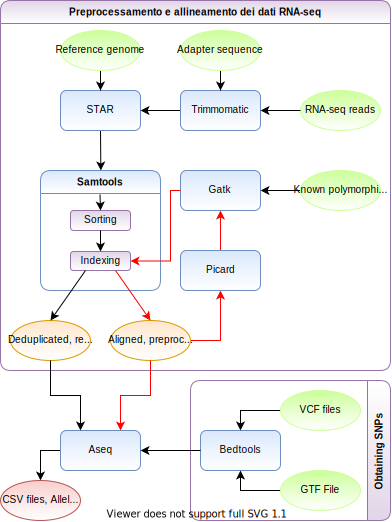
\includegraphics[scale=0.]{pipeline.png}
    \caption{Pipeline}
  \end{figure}
  \section{Dati disponibili}
  \label{sec:dati}

    \subsection{Sequenze biologiche}
    \label{subsec:fastq}
    Descrizione dei fastq.

    \subsection{Genoma di riferimento}
    \label{subsec:star-gen}
    Descrizione del genoma di riferimento.

    \subsection{Variant call}
    \label{subsec:vcf}
    Descrizione dei vcf.

    \subsection{Struttura dei geni}
    \label{subsec:gtf}
    Descrizione del gtf.

  \section{Troncatura e allinamento}
  \label{sec:trimm_star}
  Descrizione del processo e perch\`e viene fatto.

    \subsection{Troncatura}
    \label{subsec:trimm}
    Trimmomatic, cosa fa come \`e stato usato.

    \subsection{Allineamento}
    \label{subsect:star}
    STAR, cosa fa come \`e stato usato.

    \subsection{Ordinamento}
    \label{subsec:sorting}
    SAMTOOLS SORT cosa fa come \`e stato usato.

    \subsection{Indicizzazione}
    \label{subsec:indexing}
    SAMTOOLS index cosa fa come \`e stato usato.

  \section{Deduplicazione, riallinamento e recalibrazione}
  \label{sec:recalibration}
  Descrizione del processo e perch\`e viene fatto

    \subsection{Deduplicazione}
    \label{subsec:dedup}
    Come sopra.

    \subsection{Riallineamento e recalibrazione}
    \label{subsec:recalibration}
    Come sopra.

  \section{Ottenere le varianti alleliche}
  Intersezione tra VCF e GTF.

  \section{Ottenere i dati delle frazioni alleliche}
  \label{sec:aseq}
  ASEQ cosa fa come viene usato.


    \subsection{Filtrare le frazioni alleliche}
    \label{subsec:filter}
    Condizioni di filtraggio per i risultati di ASEQ.

  \section{Ottenere gli SNP nel 3'-UTR}
  \label{sec:threeprime}
  Filtraggio del gtf e intersezione con i VCF
